\documentclass{beamer}
\usepackage[utf8]{inputenc}

\usetheme{Madrid}
\usecolortheme{default}
\usepackage{amsmath,amssymb,amsfonts,amsthm}
\usepackage{txfonts}
\usepackage{tkz-euclide}
\usepackage{listings}
\usepackage{adjustbox}
\usepackage{array}
\usepackage{tabularx}
\usepackage{gvv}
\usepackage{lmodern}
\usepackage{circuitikz}
\usepackage{tikz}
\usepackage{graphicx}
\usepackage{multicol}

\setbeamertemplate{page number in head/foot}[totalframenumber]

\usepackage{tcolorbox}
\tcbuselibrary{minted,breakable,xparse,skins}



\definecolor{bg}{gray}{0.95}
\DeclareTCBListing{mintedbox}{O{}m!O{}}{%
  breakable=true,
  listing engine=minted,
  listing only,
  minted language=#2,
  minted style=default,
  minted options={%
    linenos,
    gobble=0,
    breaklines=true,
    breakafter=,,
    fontsize=\small,
    numbersep=8pt,
    #1},
  boxsep=0pt,
  left skip=0pt,
  right skip=0pt,
  left=25pt,
  right=0pt,
  top=3pt,
  bottom=3pt,
  arc=5pt,
  leftrule=0pt,
  rightrule=0pt,
  bottomrule=2pt,
  toprule=2pt,
  colback=bg,
  colframe=orange!70,
  enhanced,
  overlay={%
    \begin{tcbclipinterior}
    \fill[orange!20!white] (frame.south west) rectangle ([xshift=20pt]frame.north west);
    \end{tcbclipinterior}},
  #3,
}
\lstset{
    language=C,
    basicstyle=\ttfamily\small,
    keywordstyle=\color{blue},
    stringstyle=\color{orange},
    commentstyle=\color{green!60!black},
    numbers=left,
    numberstyle=\tiny\color{gray},
    breaklines=true,
    showstringspaces=false,
}
%------------------------------------------------------------
%This block of code defines the information to appear in the
%Title page
\title %optional
{Probability-3.0.30}
\date{\today}


\author 
{Josyula G S Avaneesh - EE25BTECH11030}



\begin{document}



\frame{\titlepage}
\begin{frame}{Question}
Two cards are drawn at random in succession,with replacement, from a deck of 52 well shuffled cards. Probability of getting both ‘Aces’ is
\begin{enumerate}
\begin{multicols}{4}
    \item $\frac{1}{169}$
    \item $\frac{2}{169}$
    \item $\frac{1}{13}$
    \item $\frac{2}{13}$
\end{multicols}
\end{enumerate}
\end{frame}


\begin{frame}{Theoretical Solution}

When dealing with probability, the phrase ``with replacement'' means that after the first card is drawn, it is put back into the deck, resetting the deck to its original state before the second draw. Therefore, the two draws are \textbf{independent events}.
\end{frame}

\begin{frame}{Theoretical Solution}

\textbf{Step 1: Probability of the first event}
A standard deck has 52 cards, and there are 4 Aces in the deck. Let $P(A_1)$ be the probability of drawing an Ace on the first draw.
\[
P(A_1) = \frac{\text{Number of Aces}}{\text{Total number of cards}} = \frac{4}{52} = \frac{1}{13}
\]

\end{frame}


\begin{frame}{Theoretical Solution} 
\textbf{Step 2: Probability of the second event}
Because the first card is replaced, the deck again has 52 cards with 4 Aces. Let $P(A_2)$ be the probability of drawing an Ace on the second draw.
\[
P(A_2) = \frac{4}{52} = \frac{1}{13}
\]
\end{frame}

\begin{frame}{Theoretical Solution}
\textbf{Step 3: Combined probability}
Since these are independent events, the probability of both events happening in succession is the product of their individual probabilities.
\begin{align*}
P(\text{Both Aces}) &= P(A_1) \times P(A_2) \\
P(\text{Both Aces}) &= \frac{1}{13} \times \frac{1}{13} = \frac{1}{169}
\end{align*}

\vspace{0.5cm}
\noindent \textbf{Correct Answer:} a) 1/169

\end{frame}


\begin{frame}[fragile]
    \frametitle{Python Code}
    \begin{lstlisting}
import random
import matplotlib.pyplot as plt
import numpy as np

#If N trials are given then this function finds experimental probability in those N trials
def simulate_aces(num_trials):
    deck = ['Ace'] * 4 + ['Other'] * 48
    success_count = 0
    
    for _ in range(num_trials):
        first_draw = random.choice(deck)
        second_draw = random.choice(deck)
        
        if first_draw == 'Ace' and second_draw == 'Ace':
            success_count += 1
            
    return success_count / num_trials



\end{lstlisting}
\end{frame}

\begin{frame}[fragile]
    \frametitle{Python Code }
    \begin{lstlisting}
# 1. Generate N values: 70 points between 100 and 100,000 logarithmically spaced

N_values = np.logspace(np.log10(100), np.log10(100000), num=70, dtype=int)

# 2. Sweep the experimental probability
experimental_probs = []
theoretical_prob = 1 / 169

print("Running 70 simulations. This might take a few seconds...")
for n in N_values:
    prob = simulate_aces(n)
    experimental_probs.append(prob)

\end{lstlisting}
\end{frame}

\begin{frame}[fragile]
    \frametitle{Python Code }
    \begin{lstlisting}
# 3. Create the plot
plt.figure(figsize=(10, 6))

# Plot discrete points for the experimental values
plt.scatter(N_values, experimental_probs, color='blue', label='Experimental Probability', zorder=5)

# Plot a continuous horizontal straight line for the theoretical value
plt.axhline(y=theoretical_prob, color='red', linestyle='--', linewidth=2, 
            label=f'Theoretical Probability (1/169 ≈ {theoretical_prob:.5f})', zorder=4)

# Apply Bode plot style formatting (Logarithmic X-axis)
plt.xscale('log')

\end{lstlisting}
\end{frame}

\begin{frame}[fragile]
    \frametitle{Python Code }
    \begin{lstlisting}
# Formatting to make it readable and professional
plt.title('Convergence of Probability: Drawing Two Aces (With Replacement)')
plt.xlabel('Number of Trials (N) - Logarithmic Scale')
plt.ylabel('Probability')
plt.grid(True, which="both", linestyle="--", alpha=0.6) # Adds gridlines for both major and minor log ticks
plt.legend()
plt.savefig("../plot.png")

# Display the plot
plt.show()

\end{lstlisting}
\end{frame}


\begin{frame}{Plot}
    \centering
    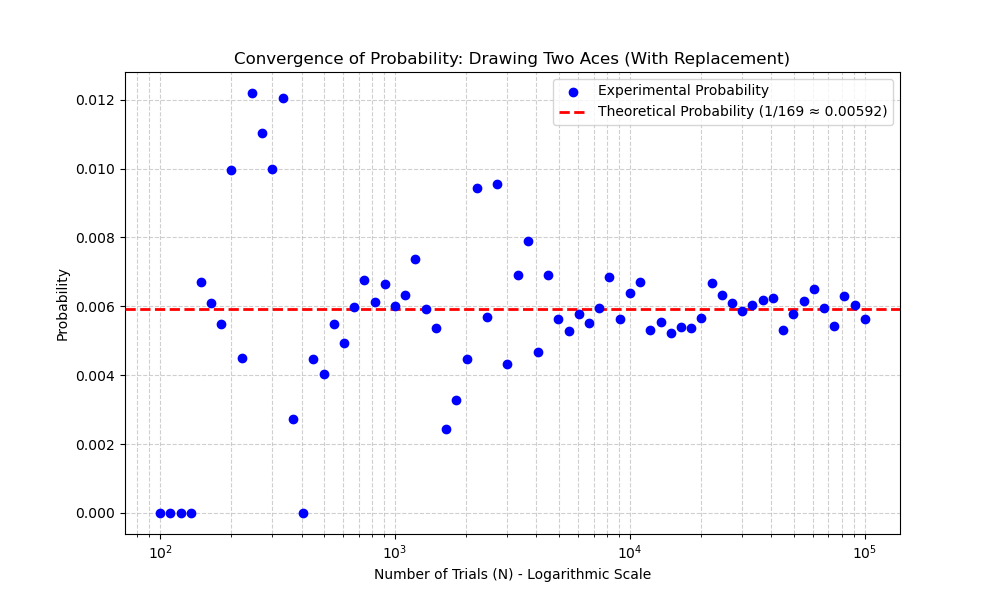
\includegraphics[width=\columnwidth, height=0.8\textheight, keepaspectratio]{plot.png}     
\end{frame}


\end{document}